\section{はじめに}
近年の人工知能(AI)の目覚ましい発展は、まさに「ニューラルネットワーク」という技術によって牽引されてきました。スマートフォンが顔を認識したり、音声アシスタントが言葉の意味を理解したり、あるいはAIが美しい絵画や自然な文章を生成したり――私たちが日常で「すごい」と感じるAIの多くが、このニューラルネットワークを基盤として動いています。

とはいえ、「ニューラルネットワーク」と聞くと、難解な数式や複雑な理論を思い浮かべてしまう人も少なくないでしょう。

でも、安心してください。本稿の目的は、数学的な細部に立ち入ることではありません。私たちが共有したいのは、この技術の「どこが面白いのか」、そして「なぜここまで強力なのか」という「直感」です。

本稿は、\textbf{「AI という言葉は知っているが、体系的に学んだことはない」}という方に向けた、やさしい入門ガイドです。専門的な知識がなくても読み進められるよう、基本的な概念から丁寧に解説していきます。

\section{生物の神経細胞から着想を得たモデル}
ニューラルネットワークの最初のアイデアは、非常にシンプルで、私たちの身近にあるものから着想を得ています。それは、生物の脳に存在する\textbf{ニューロン(神経細胞)}です。

私たちの脳内では、ニューロンが複雑なネットワークを形成しています。個々のニューロンは、他のたくさんのニューロンから電気的な信号を受け取ります。そして、受け取った信号の合計が、ある一定の「しきい値(閾値)」を超えると、そのニューロンは「発火(興奮)」し、次のニューロンへと今度は自らが信号を送るのです。

この仕組みを、ごくごくシンプルに数学的なモデルとして置き換えてみましょう。

\begin{enumerate}
    \item 複数の入力(信号)を受け取る。
    \item それらを合計する。
    \item 合計が「しきい値」を超えたら「1」(発火)を、超えなければ「0」(発火しない)を出力する。
\end{enumerate}

たったこれだけです。これが、人工ニューラルネットワークの原点であり、出発点です。

ここで重要な直感が生まれます。私たちの「知能」や「記憶」は、決して一つの万能なニューロンが担っているわけではありません。むしろ、比較的単純な働きをする「多数の素朴な処理ユニット」が、お互いに結びつき、チームとして連携することで、全体として非常に高度な知性が生まれるのではないか、という考えです。

この「チームワーク」こそが知性の本質である、という考えは、生物学的な事実とも一致します。例えば、あるサッカーチームが1年間練習して強力なチームワークを築いたとします。もし急にメンバーの半分がルールも知らない素人と入れ替わったら、そのチームはガタガタになってしまいます。脳のニューロンが頻繁に入れ替わらないのは、この「チームワーク」、すなわちニューロン同士の安定した接続パターンこそが「記憶」や「知能」そのものだからです。

ニューラルネットワークも同じです。個々の「処理ユニット(人工ニューロン)」は単純でも、その「接続の仕方」や「連携の強さ(チームワーク)」を学習させることで、大きな知能が生まれるのです。

\section{パーセプトロン:最初のニューラルネットワーク}
この「脳の神経細胞(ニューロン)」の仕組みを、世界で初めて工学的にモデル化したものが、1950年代に考案された「パーセプトロン」です。これは、まさにAIの「ご先祖様」と呼べる存在です。

パーセプトロンの仕組みは、先ほどのニューロンのモデルとほぼ同じです。複数の入力に対し、それぞれ「重み」をかけて合計し、その値が「しきい値(あるいはバイアス)」を超えたら1、そうでなければ0を出力します。

\begin{figure}[H]
  \centering
  \begin{tikzpicture}[
    >=Stealth,
    node distance=2.2cm,
    every node/.style={font=\normalsize}
  ]
    % ノード
    \node[circle, draw, minimum size=10mm] (sum) {$\sum$};
    \node[draw, rounded corners, right=3cm of sum, minimum height=10mm, minimum width=16mm] (act) {$\varphi(\cdot)$};
    \node[right=2.5cm of act] (y) {$y$};

    % 入力(x1, x2, ..., xn)
    \node[left=4.2cm of sum, yshift=12mm] (x1) {$x_{1}$};
    \node[left=4.2cm of sum, yshift=4mm]  (x2) {$x_{2}$};
    \node[left=4.2cm of sum, yshift=-12mm] (xn) {$x_{n}$};

    % 省略記号
    \node[left=4.2cm of sum] (dots) {$\vdots$};

    % バイアス(1 → Σ, 重み b)
    \node[left=4.2cm of sum, yshift=-28mm] (one) {$1$};

    % 矢印(入力→Σ)
    \draw[->] (x1) -- node[above, pos=0.55] {$w_{1}$} (sum);
    \draw[->] (x2) -- node[above, pos=0.55] {$w_{2}$} (sum);
    \draw[->] (xn) -- node[above, pos=0.55] {$w_{n}$} (sum);
    \draw[->] (one) -- node[above, pos=0.55] {$b$} (sum);

    % Σ → 活性化 → 出力
    \draw[->] (sum) -- node[above] {$z=\sum_{i=1}^{n} w_i x_i + b$} (act);
    \draw[->] (act) -- (y);

  \end{tikzpicture}
  \caption{単一パーセプトロンの模式図(重み $w_i$,バイアス $b$,活性化 $\varphi$)}
  \label{fig:perceptron}
\end{figure}

ここで新しい言葉が2つ出てきました。「重み」と「しきい値(バイアス)」です。これらを簡単な例で考えてみましょう。

あなたが「今日は傘を持っていくべきか?」を判断する、シンプルなパーセプトロン(“傘判断”AI)になったと想像してください。

\begin{itemize}
    \item \textbf{入力}:
     
    入力1 $x_1$:「雨が降っているか?」(Yes=1, No=0)

    入力2 $x_2$:「天気予報が雨か?」(Yes=1, No=0)
    \item \textbf{重み}:
    
    「どの入力を、どれだけ重視するか」をコントロールする値です。

    重み1 $w_1$:「今、実際に降っている」(入力1)は非常に重要なので、重み5に設定。

    重み2 $w_2$:「予報」(入力2)は、まぁ重要だが外れることもあるので、重み2に設定。
    \item \textbf{しきい値(バイアス)}:

    「どれくらいで"発火"(傘を持つ)と決めるか」のボーダーラインです。

    あなたがとても慎重な人なら、しきい値を1に設定するかもしれません(予報が雨なだけで傘を持つ)。

    あなたが楽観的な人なら、しきい値を4に設定するかもしれません(予報だけでは持たず、実際に降ってきたら持つ)。
\end{itemize}

この「重み」や「しきい値」をデータ(過去の経験)から自動で調整(学習)できるようにしたのが、パーセプトロンの画期的な点でした。

しかし、この初期のパーセプトロンには大きな限界がありました。それは、「線形的にしか境界を引けない」という問題です。

先ほどの例のように、入力の“足し算”で判断できるシンプルな問題(これは「線形分離可能」と呼ばれます)は解けます。しかし、世の中の問題はもっと複雑です。

例えば、「入力1と入力2の“どちらか一方だけ”がYesの時に1(発火)になる」という、有名な「XOR問題」はこのパーセプトロンでは解けませんでした 。一本の直線では、この複雑な条件分けをどうやっても表現できなかったのです。

この“限界”の指摘は、当時のニューラルネット研究に大きな影響を与えました。もちろん、1960〜70年代に訪れた「AIの冬の時代」は、パーセプトロンの限界だけが原因ではありません。むしろ、ルールベースの記号処理AIが直面していた根本的な性能不足や計算資源の制約が、研究全体を停滞させた側面の方が大きかったと言われます。とはいえ、パーセプトロンではXORすら解けないという事実は、「より柔軟で表現力の高いモデルが必要だ」という強い問題意識を生み、のちの多層化──すなわち深層学習(ディープラーニング)へとつながる重要な伏線となりました。

\begin{figure}[H]
  \centering
  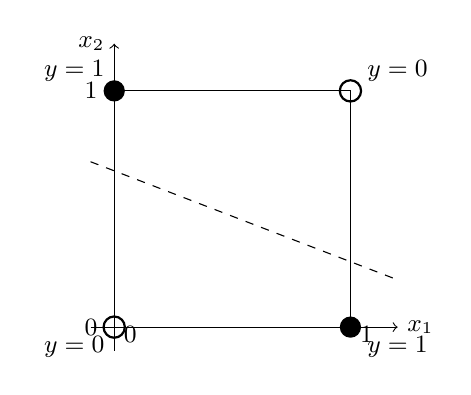
\begin{tikzpicture}[
    scale=3,
    every node/.style={font=\small}
  ]
    % 枠と座標軸
    \draw[->] (-0.1,0) -- (1.2,0) node[right] {$x_1$};
    \draw[->] (0,-0.1) -- (0,1.2) node[left] {$x_2$};
    \draw (0,0) rectangle (1,1);

    % 目盛り
    \foreach \x in {0,1}{
      \draw (\x,0) -- (\x,-0.03) node[right] {\x};
      \draw (0,\x) -- (-0.03,\x) node[left] {\x};
    }

    % XOR のデータ点
    % y=0:白抜き
    \draw[thick] (0,0) circle [radius=0.045];
    \draw[thick] (1,1) circle [radius=0.045];
    % ラベル(点と重ならないようアンカーで配置)
    \node[anchor=north east] at (0,0) {$\;y=0$};
    \node[anchor=south west] at (1,1) {$\;y=0$};

    % y=1:塗りつぶし
    \fill (1,0) circle [radius=0.045];
    \fill (0,1) circle [radius=0.045];
    % ラベル
    \node[anchor=north west] at (1,0) {$\;y=1$};
    \node[anchor=south east] at (0,1) {$\;y=1$};

    % 任意の直線(例示)
    \draw[dashed] (-0.1,0.7) -- (1.2,0.2);

  \end{tikzpicture}
  \caption{XOR の例:対角に異なるクラスが配置され、どの直線でも完全に分離できない(線形分離不可能)}
  \label{fig:xor_not_linearly_separable}
\end{figure}

\section{多層パーセプトロン(MLP)と深層学習の基本}
パーセプトロンの「XOR問題」という壁。この限界を乗り越えるために生まれたのが、\textbf{多層パーセプトロン(MLP: Multi-Layer Perceptron)}です。

アイデアは、構造を「多層化」することでした。

パーセプトロンが「入力層」と「出力層」だけだったのに対し、MLPはその間に\textbf{「隠れ層(Hidden Layer)」}と呼ばれる新しい層を挿入しました。

\begin{figure}[H]
  \centering
  \begin{tikzpicture}[
    >=Stealth,
    neuron/.style={circle, draw, minimum size=9mm},
    every node/.style={font=\small},
    conn/.style={->, shorten >=1pt, shorten <=1pt}
  ]

    %=== X(横位置) ===%
    \def\xin{0}
    \def\xhid{4}
    \def\xout{8}

    %=== 入力層(縦配置) ===%
    \node[neuron] (x1) at (\xin,  2.4) {$x_1$};
    \node[neuron] (x2) at (\xin,  0.8) {$x_2$};
    \node[neuron] (x3) at (\xin, -0.8) {$x_3$};
    \node            at (\xin, -2.0) {$\vdots$};
    \node[neuron] (xn) at (\xin, -3.2) {$x_n$};

    % 層タイトル(被らないよう十分上に)
    \node[font=\bfseries] at (\xin, 3.25) {入力層};

    %=== 隠れ層(1層) ===%
    \node[neuron] (h1) at (\xhid,  2.0) {$h_1$};
    \node[neuron] (h2) at (\xhid,  0.7) {$h_2$};
    \node[neuron] (h3) at (\xhid, -0.6) {$h_3$};
    \node            at (\xhid, -1.8) {$\vdots$};
    \node[neuron] (hm) at (\xhid, -3.0) {$h_m$};

    \node[font=\bfseries] at (\xhid, 3.25) {隠れ層(活性化 $\varphi$)};

    %=== 出力層 ===%
    \node[neuron] (y)  at (\xout, 0.7) {$y$};
    \node[font=\bfseries] at (\xout, 3.25) {出力層};

    %=== 入力→隠れ(全結合) ===%
    \foreach \xinode in {x1,x2,x3,xn}{
      \foreach \hnode in {h1,h2,h3,hm}{
        \draw[conn] (\xinode) -- (\hnode);
      }
    }

    %=== 隠れ→出力(全結合) ===%
    \foreach \hnode in {h1,h2,h3,hm}{
      \draw[conn] (\hnode) -- (y);
    }

    %=== ラベル(図のさらに上に逃がす) ===%
    \node at ({(\xin+\xhid)/2}, 3.85)
      {全結合層( $W^{(1)}$, $b^{(1)}$)};
    \node at ({(\xhid+\xout)/2}, 3.85)
      {全結合層( $W^{(2)}$, $b^{(2)}$)};

    % 数式メモ
    \node at (\xhid, -4.0) {$h=\varphi(W^{(1)}x+b^{(1)}),\; y=\psi(W^{(2)}h+b^{(2)})$};

  \end{tikzpicture}
  \caption{多層パーセプトロン(MLP)の模式図。入力層→隠れ層(活性化 $\varphi$)→出力層。各層は全結合され、重みとバイアスが学習で更新される}
  \label{fig:mlp_one_hidden}
\end{figure}
この「隠れ層」が何を解決したのか。再び、例え話で考えてみましょう。

あなたは、画像に写っているのが「猫」か「猫でない」かを判定するAI(の出力層、つまり最終決定者)だとします。

まず、入力層から送られてくるのは何万個ものピクセルの色情報です。しかし、生のピクセル値だけを眺めても、「右上の点が茶色で、中央が黒で……」といった断片的な情報の寄せ集めにすぎず、そこから“猫”という概念を直接読み取るのは困難です。これは、パーセプトロン(隠れ層なし)が抱える「複雑なパターンを捉えられない」という限界そのものです。

そこで登場するのが、隠れ層という“専門家チーム”です。隠れ層の各ニューロンは、生のピクセルをそのまま扱うのではなく、自分の得意分野に応じて情報をまとめ上げる役割を担います。

\begin{itemize}
    \item ニューロンA:「私は尖った耳の特徴を検出します」
    \item ニューロンB:「私はヒゲのパターンを見るのが得意です」
    \item ニューロンC:「私は丸い目に反応します」
\end{itemize}

こうして隠れ層は、生のピクセルからより抽象的で意味のある“特徴”を抽出し、「尖った耳:90%」「ヒゲ:70%」「丸い目:85%」といった形に変換してくれます。あなた(出力層)は、もはや膨大なピクセル値を直接扱う必要はなく、こうした中間的な“猫らしさ”の指標を組み合わせて、最終的な判断ができるようになります。

これなら、あなた(出力層)の仕事は簡単です。「耳とヒゲと目のスコアが高いから、これは“猫”だ」と、はるかに賢い判断ができます。

これが、多層パーセプトロン(MLP)の核心です。

\begin{enumerate}
    \item 層を深くする(隠れ層を増やす)ことで、より複雑なパターン(ピクセル→耳→猫)を表現できるようになりました。
    \item 各層が異なるレベルの抽象化を担うことで、全体として強力な知能が生まれます。人間が「耳」や「ヒゲ」といった"良い特徴量"を必死に設計しなくても、モデル(隠れ層)自身がデータから自動で"良い特徴"を学んでくれるようになりました。
    \item そして、隠れ層のニューロン(専門家)が「発火」するかどうかを決める際、\textbf{活性化関数(Activation Function)}と呼ばれる仕組みが使われます。
\end{enumerate}

特に重要なのが3番目の「活性化関数」です。もし隠れ層が、入力された情報をただ足し合わせて次の層に渡すだけ(線形)なら、層をどれだけ重ねても、結局は1枚のパーセプトロンと同じことしかできません。

そこで、各ニューロンは受け取った信号に対し、「非線形(カクンと曲がる)」な処理を加えます。現在、最も標準的に使われる\textbf{ReLU(レル)}という活性化関数は、驚くほどシンプルです。「入力がマイナスなら0(発火しない)、プラスならそのまま通す」たったこれだけです。

この単純な「カクン」という非線形性が、ニューラルネットワークに複雑な境界線を引く能力を与え、XOR問題をはじめとする現実の複雑な問題を解く力を与えたのです。

そして、この「隠れ層」を何層にも何層にも深く重ねて、より高度な特徴を学習させよう、というアイデアが、現在の\textbf{深層学習(ディープラーニング)}の基本構造となっています。

\section{学習の仕組み:誤差逆伝播法}
MLPという強力な「構造」を手に入れました。では、この構造(隠れ層の専門家チーム)は、どうやって「学習」するのでしょうか? どうすれば、ピクセル情報から「耳」を見つけ出すような“優秀な専門家”に育ってくれるのでしょうか?

その答えが、ニューラルネットワークの学習を可能にする、最も中心的で美しいアイデア、\textbf{「誤差逆伝播法(Backpropagation)」}です。

ニューラルネットワークは、文字通り「間違いから学習する」仕組みを持っています。

先ほどの「猫」の例で、学習のプロセスを直感的に見てみましょう。

\begin{enumerate}

  \item \textbf{予測(順伝播)}:

  まず、ネットワークに「猫」の画像を入力します。  
  ネットワークは、現在の(まだ学習途中の)重みに基づいて、
  「入力層」→「隠れ層」→「出力層」へと信号を順に伝えながら予測を計算します。  
  たとえば、AI が「犬 70\%・猫 30\%」と予測したとします。

  \item \textbf{誤差の計算}:

  人間側は「正解は猫 100\%だよ」と教えてあげます。  
  AI は、自分の予測(猫 30\%)と正解(猫 100\%)を比較し、  
  どれくらい間違っていたか=\textbf{誤差}を計算します。  
  「うわ、70\% も外していた!」というイメージです。


  \item \textbf{逆伝播(Backpropagation)}:

  計算された誤差は、今度は「出力層」から「隠れ層」へ、  
  さらに「入力層」へと逆向きに伝わっていきます。  
  このとき誤差は、  
  「どのニューロンがどれだけ間違いに貢献したか」  
  という“責任”の大きさに応じて分配されます。

  出力層(あなた):「犬と判断したのは大間違いだった!」  

  隠れ層(専門家):「私の“垂れた耳”レポートがミスに大きく関与してしまった…」  
  「私の“ヒゲ”レポートは、あまり関係なかったかも…」

  \item \textbf{重みの調整(更新)}:

  間違いに強く関わった接続(重み)は、  
  \textbf{次は少しでも誤差が減る方向}へと微調整されます。  

  “垂れた耳”と“犬”を結びつけていた重みは少し弱くなり、  
  “尖った耳”と“猫”を結びつけていた重みは少し強くなります。

\end{enumerate}

この1〜4のプロセスを、何万、何億という膨大なデータ(たくさんの猫や犬の画像)で繰り返します。この「間違い」と「修正」のサイクルこそが、ニューラルネットワークの「学習」です。

では、具体的に「どちらの方向に」「どれくらい」重みを調整すれば、間違い(誤差)が減るのでしょうか?

その調整方法を教えてくれるのが、\textbf{勾配降下法(Gradient Descent)}です。

これはよく、\textbf{“霧の中の山下り”}に例えられます。

\begin{itemize}
    \item あなたは今、深い霧に包まれた広大な山の、どこかの斜面に立っています。
    \item あなたの\textbf{「現在の位置」は、ネットワークの「現在の重みの組み合わせ」}です。
    \item あなたの\textbf{「標高」は、ネットワークの「現在の誤差の大きさ」}です。
    \item あなたの\textbf{「目的」は、山の一番低い場所、「谷底(誤差が最小になる地点)」}にたどり着くことです。

\end{itemize}

霧が深くて谷底は見えません。さあ、どうしますか?

最も賢明な方法は、自分の足元を調べることです。地面の\textbf{「傾き(勾配)」を調べ、今いる場所で「最も急な下り坂」になっている方向を見つけます。そして、その方向に「ほんの一歩だけ」進みます。}

一歩進んだら、またその場で最も急な下り坂を探し、また一歩進む。これを何千回、何万回と繰り返すのです。そうすれば、いつかは谷底(最適な重み)にたどり着けるはずです。

こうして、勾配(傾き)を手がかりに誤差の情報を逆向きに伝えながら、重みという“現在地”を少しずつ更新していく──これが、誤差逆伝播と勾配降下法によってニューラルネットワークが学習する仕組みの核心です。

実際には、データ全体を使って一歩(バッチ勾配降下法)、あるいは少量のデータで素早く一歩(ミニバッチ勾配降下法、確率的勾配降下法)など、山の下り方にも様々な工夫があります。特に確率的勾配降下法(SGD)は、ノイズが多くて不安定な(ジグザグに進む)反面、巨大なデータセットでも高速に学習でき、局所的な谷(局所最適解)から脱出しやすいというメリットがあります。

\section{おわりに}
以上が、ニューラルネットワークの基本的な仕組みと学習方法の概要です。
見てきたように、ニューラルネットワークは、単純な計算を行う多数のユニットが層をなし、そのつながりの強さ(重み)を調整しながら、少しずつ正解に近づいていく仕組みです。隠れ層は生のデータから意味のある特徴を抽出し、誤差逆伝播は「どの部分がどれだけ間違いに関わったのか」をネットワーク全体に伝え、勾配降下法は「次にどちらへ進めばよいか」を教えてくれます。

こうした素朴なステップの積み重ねが、やがて“猫”や“犬”といった複雑な概念さえ自動で学び取る力へとつながります。私たちが日常で目にする高度なAIの裏側には、この静かで着実な試行錯誤の連続が息づいているのです。

ただ、ここまで扱ってきたモデルには、ひとつ意外な前提があります。それは、\textbf{ニューラルネットワークは本来「決定論的」に動作する}という点です。同じ入力を与えれば、いつも同じ答えを返す──これは数学的には自然ですが、実世界のあり方とは少し違います。

というのも、私たちが相手にしている自然現象は、たいていの場合、\textbf{揺らぎ}や\textbf{不確実性}を内包しています。観測値はノイズを含み、物理現象は確率的にばらつき、生命現象に至っては再現性そのものが確率論的です。世界は“ひとつの答え”を返すのではなく、むしろ“ゆらいだ分布”として姿を見せます。

その意味で、決定論的なニューラルネットワークだけでは、自然のふるまいを本質的に捉えきれないのではないか──そんな疑問も生まれてきます。

こうした問題意識から生まれたのが、\textbf{ベイズ的ニューラルネットワーク(Bayesian Neural Network; BNN)}という考え方です。BNNでは重みを固定の値としてではなく「確率分布」として扱い、モデル自身が「どれくらい確信しているか」まで推論します。予測の幅や不確実性そのものを扱える点で、自然界の“ゆらぐ”構造により近い表現とも言えます。

本稿では詳細に立ち入りませんが、もしニューラルネットワークと自然現象の関係に興味があるなら、この「確率的な知性」のアプローチはきっと刺激的に映るはずです。
決定論的なモデルの上に、どこまで“自然のゆらぎ”を重ねられるのか──その先には、AIが世界をどう捉えうるのかという、静かな問いが立ち上がります。
